\section{Runtime and causal service}
\label{sec:runtime}

The persistent service completed every update in its five-second paced replay and preserved numerical parity, but it missed the 20\,ms response target. The 95th percentile was 29.14\,ms. The distinction between model execution and delivery of a complete prediction explains why a faster inner kernel is not enough to meet the deadline.

\begin{figure}[H]
\centering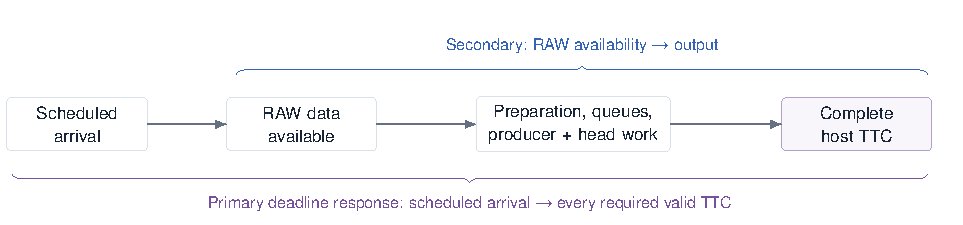
\includegraphics[width=\linewidth]{figures/rev_runtime_clock.pdf}
\caption{\textbf{Response clocks for one query.} Deadline response starts at scheduled arrival; the secondary clock starts when RAW data become available. Both stop when all required TTC outputs reach the host.}
\label{fig:runtime-clocks}
\end{figure}

\subsection{Latency measurement boundaries}

Earlier timing experiments measured different parts of the computation. V18 used warm raw-sensor queries with its original producer batching. The final test12 diagnostics timed a prepared eager path, and the EvTTC transfer measured adapter wall time, including preparation and cache behavior. Hardware and inputs also varied. We report these measurements separately and use the scheduled-arrival clock for the deadline test below. The saved timing record contains aggregate statistics, so the analysis uses quantiles and deadline counts rather than reconstructing a per-arrival distribution.

The service reduced repeated work by preparing RGB within the object region, extending event prefixes incrementally, and reusing reverse-transport summaries exactly. It also combined top-$k$ normalization with native query graphs and parallel branches, overlapping event execution with RGB preparation. RGB features were reused; event encodings were recomputed. A separate diagnostic verified all 462 recorded calls to the prepared transport component. \evidence{L41}

Numerical checks rejected several faster alternatives. Compiled transport arithmetic changed the final TTC on sensitive examples despite agreeing on most others. Processing smaller event packets preserved the tested state buffers, representations, and final predictions, but that experiment did not time the computation or run a 200\,Hz source through the paced service. It established a viable numerical path for a later timing experiment. \evidence{L42}

\subsection{Paced-service latency at 50 Hz}

We ran the replay on an NVIDIA GeForce RTX 5070 Ti Laptop GPU using Python 3.11.15 and PyTorch 2.11.0+cu128, built with CUDA 12.8. Computation used FP32 with TF32 disabled, two PyTorch CPU threads, eight RGB preparation workers, and a queue capacity of two. Model loading, synthetic shape priming, and initialization from preceding history finished before measured arrivals. Table~\ref{tab:runtime-setup} gives these setup intervals and the parity tolerance. \evidence{L40,R02}

The five-second replay processed 250 single-object updates from preloaded RAW data accessible only to the CPU feeder. All updates completed with zero drops and zero source errors, and independent post-run checks confirmed TTC parity. Nevertheless, 200 scheduled arrivals found earlier work unfinished. Of the 250 responses, 201 met or exceeded 20\,ms. Scheduled-arrival latency reached 29.14\,ms at p95, 32.41\,ms at p99, and 35.33\,ms at maximum. Starting the clock after RAW data became available gave a lower p95 of 25.25\,ms. \evidence{L40}

The measurement excludes disk I/O and covers one object over five seconds. It therefore leaves physical-camera input, sixty-second operation, and larger object counts for further testing. Failed replays remain in separate reports, including dropped updates and rapid error acknowledgements. We count latency only for successful TTC outputs, so a fast acknowledgement cannot improve the prediction-latency summary.

\begin{figure}[t]
\centering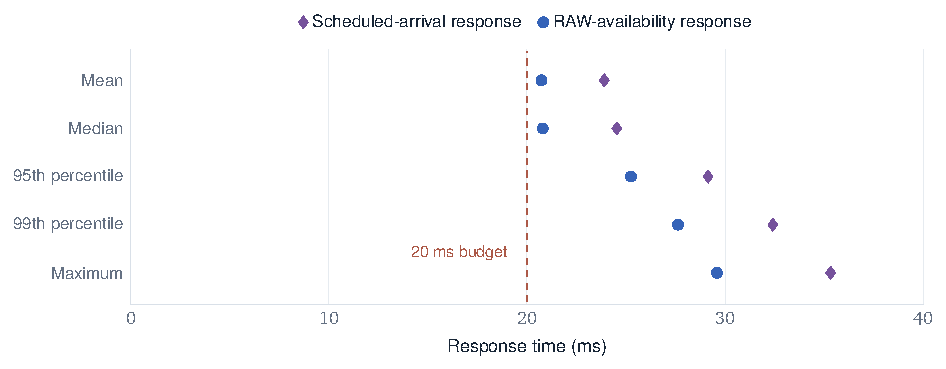
\includegraphics[width=0.98\linewidth]{figures/rev_runtime.pdf}
\caption{\textbf{Response-time summaries for 250 completed updates.} Scheduled-arrival latency has a p95 of 29.14\,ms. Of the 250 responses, 201 (80.4\%) meet or exceed 20\,ms. The second clock begins when RAW data become available. \evidence{L40}}
\end{figure}
\FloatBarrier
